\begin{figure}
	\centering
	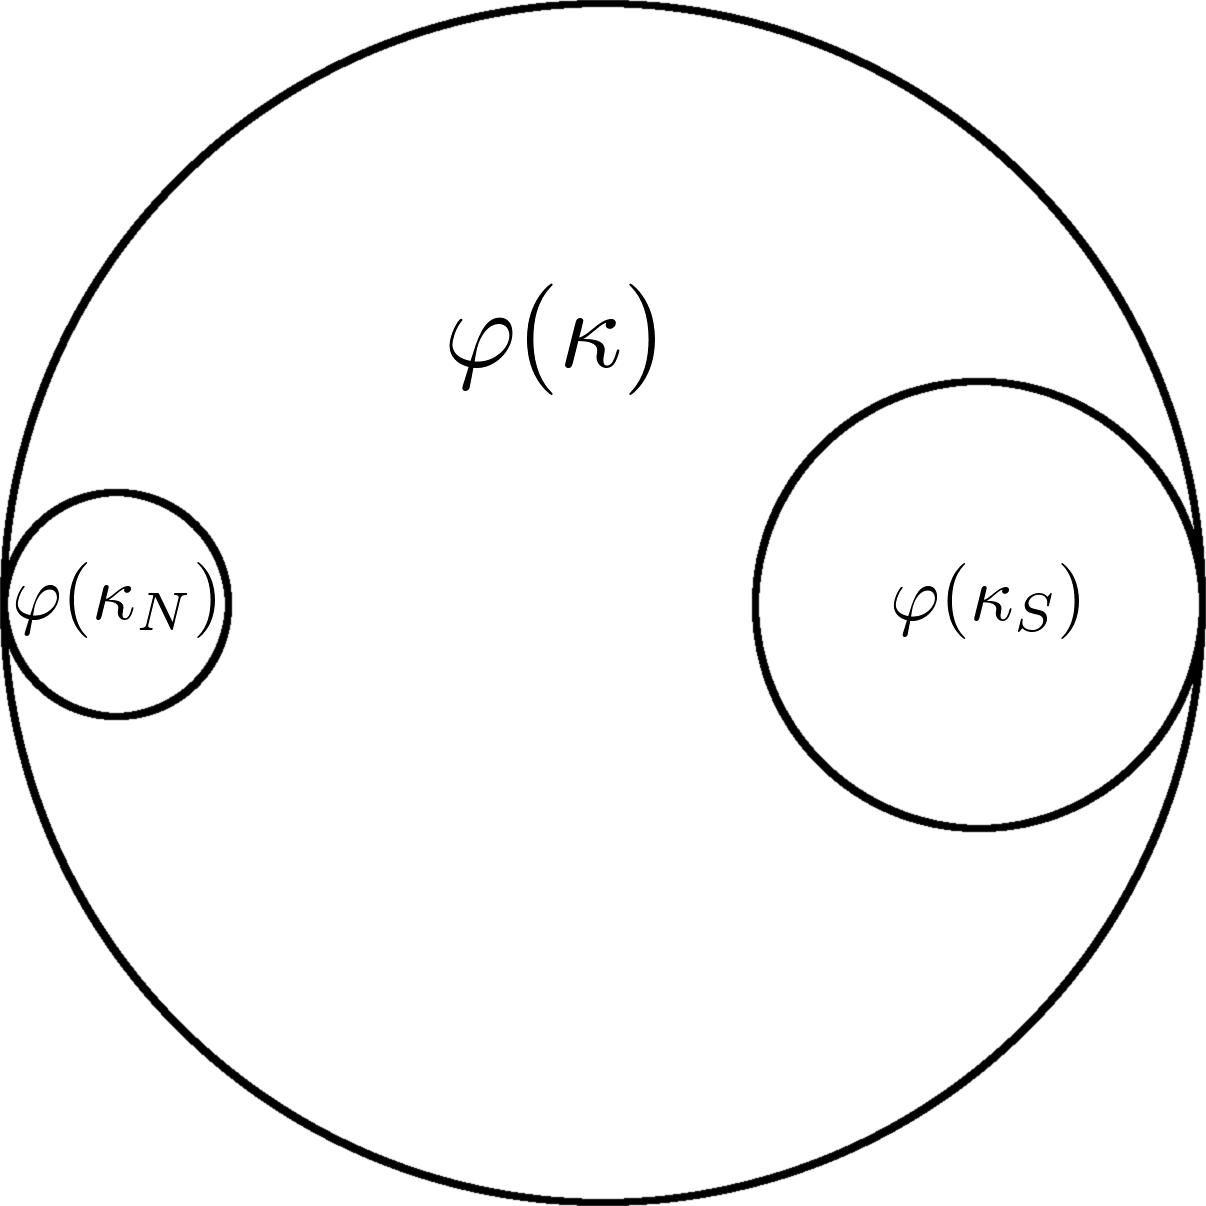
\includegraphics[width=.4\textwidth]{figs/differentkappa}\\[1.5em]
	\caption{ The construction used in \Cref{thm:convhull}. }
	\label{fig:caphr}
\end{figure}

\begin{theorem}
	\label{thm:convhull}
	Let $A$ be a region on the sphere.  Then there exist two regions $\kappa'_N,\kappa'_S\subset A$ such that the convex hull scores of $\kappa'_N$ and $\kappa'_S$ are equal on the sphere, but under the gnomonic projection $\varphi$, the convex hull score of $\kappa'_S$ is strictly greater than that of $\kappa'_N$. 
\end{theorem}

\begin{proof}
  First, since $A$ is a region, we can find some cap $\kappa$ inside
  of $A$ such that the center of $\kappa$ is not the south pole of the
  sphere, and the north pole is exterior to $\kappa$.  This cap is
  bisected by a line of longitude, in particular the great circle
  which passes through the two poles and the center of $\kappa$.  This
  line of longitude meets $\kappa$ at exactly two points, and we call
  $p_N$ the point closer to the north pole and $p_S$ the point closer
  to the south pole.
	
  Choose some $r$ strictly less the radius of $\kappa$ and let
  $\kappa'_S$ be the region constructed by deleting a cap of radius
  $r$ from the interior of $\kappa$ tangent at $p_S$.  Construct
  $\kappa'_N$ analogously by deleting a cap of radius $r$ tangent at
  $p_n$. Observe that the convex hull scores of $\kappa'_N$ and
  $\kappa'_S$ are identical, since each has the boundary of $\kappa$
  as its smallest bounding cap and both convex hulls have the same
  area.
	
  We now consider the images of $\kappa'_N$ and $\kappa'_S$ under the
  gnomonic projection $\varphi$.  Since $\varphi$ preserves points of
  tangency, containment, and sends every cap to an ellipse, the images
  $\varphi(\kappa'_N)$ and $\varphi(\kappa'_S)$ are both regions which
  are ellipses with a smaller ellipse, tangent to a point on the
  circumference, deleted.  Furthermore, since the boundary of $\kappa$
  was the smallest bounding cap of both regions on the sphere, the
  image of the boundary of $\kappa$ under $\varphi$ is the smallest
  bounding circle of the images of these regions in the plane.
	
  We can now observe that these two regions in the plane do not have
  the same convex hull score.  Both have the same bounding ellipse,
  which is their convex hulls, but $\varphi(\kappa'_N)$ is strictly
  smaller than $\varphi(\kappa'_S)$.  This is because the gnomonic
  projection distorts areas in a way such that regions further from
  the south pole have their areas magnified more than the same region
  closer to the south pole.  If the regions in question are
  sufficiently small, letting $\theta$ denote the polar angle at which
  we consider a small cap on the sphere, a cap of radius $r$ will be
  sent to an ellipse with a major axis (along the line through the
  center of the ellipse and the origin) of length roughly
  $r/\sin^2{\theta}$\zs{check  this}, and a minor axis of length
  $r/\sin{\theta}$, and a straightforward examination of this as
  a function of $\theta$ shows that it grows faster as $\theta$
  increases.
	
  Since $\varphi(\kappa'_N)$ fills a smaller fraction of the bounding
  ellipse than $\varphi(\kappa'_N)$ does, its convex hull score is
  strictly worse, and the gnomonic projection does not preserve convex
  hull scores.
\end{proof}
